\begin{frame}
    \frametitle{Method of Fragments}
    {\color{hlfont}Hand-waving} is problematic:

    \hspace{2em}\str{Ahmed paints. He is quiet.}
    {$\quad\stackrel{?}{\leadsto}\quad$ \color{logicfont} $p(a)\wedge q(a)$}

    \vspace{1.2em}
    {\color{hlfont}Montague}: Specify
    \begin{itemize}
        \item grammar,\com{fixes NL subset}
        \item target logic,
        \item semantics construction.\com{maps parse trees to logic}
    \end{itemize}

    {
        \centering
        \vspace{0.3em}
        {\itshape\footnotesize Example from~\cite{Montague:tptoqi73}}

        \vspace{0.2em}\fbox{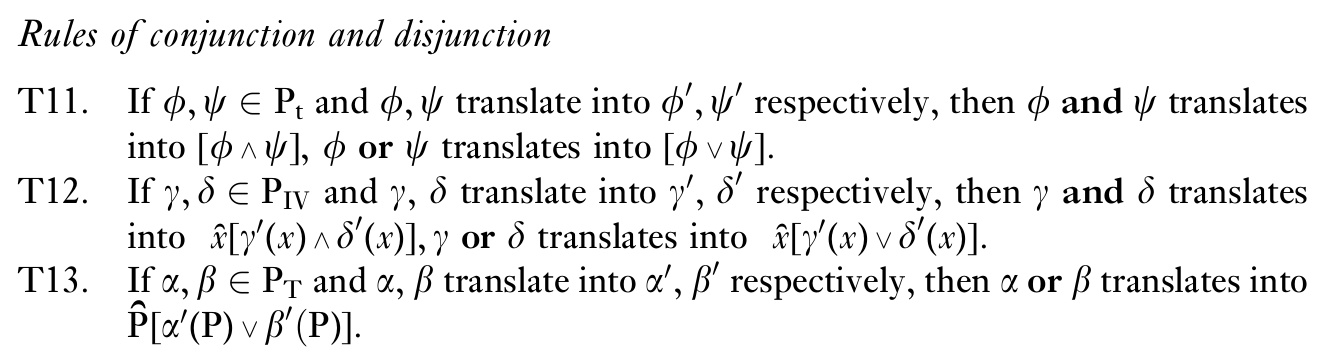
\includegraphics[trim=0 0 0 80,clip,width=0.7\textwidth]{fig/montague-tptoqioe.png}}

        \vspace{1.2em}
        Claim: That doesn't scale well $\leadsto$ \textbf{We need {\color{hlfont}prototyping}!}
    }

    % \newcommand\VP{\text{\upshape\tiny VP}}
    % \hspace{2em}$\llbracket\text{\strplain{$P_{\VP}$ and $Q_{\VP}$}}\rrbracket_{\VP} = \lambda x. \llbracket\text{\strplain{$P_{\VP}$}}\rrbracket(x) \wedge \llbracket\text{\strplain{$Q_{\VP}$}}\rrbracket(x)$
\end{frame}
